% !TEX root = ../main.tex

\chapter{Background}
\label{ch:background}
This chapter is about what steps were involved to determine which learned index structure was worth the effort of further exploration. As a starting point, this was achieved by running and evaluating the SOSD benchmark from \cite{sosd-neurips} on a local system. Further, as a second indicator, by looking at what different learned index strucures make use of in terms of complexity during their learning phases or more importantly what level of complexity and what programming concepts are needed during a lookup.\newline
Finally this chapter looks at the basic capabilities and limitations of the P4 language, especially in regard to what the language offers that could be used as an advantage for learned index structures or on the other hand which important concepts are potentially missing.

\section{SOSD}
In this first section the goal is to analyse the results of the SOSD benchmark. For doing so my work consisted of understanding the code by myself as well as comparing our local results with what is given by the authors. To do so the initial goal was to reproduce Table 2 from \cite{sosd-neurips}, which gave the result shown in \ref{fig:sosd_lookups}. Important to mention for these figures is that to obtain these results, the benchmark runs different pareto runs for each algorithm on each dataset from which the optimal run with respect to the three metrics lookup time, build time and index size is selected. Now at this given point in time it was important for this work to take note of the fact that learned index structures effectively can outperform traditional index structures when tuned properly. This means that for now the assumption that the ability to train an algorithm on a given dataset can translate to faster lookup times is given. With respect to the other metrics, this results in a tradeoff between either slower lookup times but no build time or instead spending time upon build as pointed out in \ref{fig:sosd_builds} to then gain with faster lookups.

% probably need to write more here, analyse more how the algorithms work with repsect to speed / index size

\begin{figure}[ht]
\centering
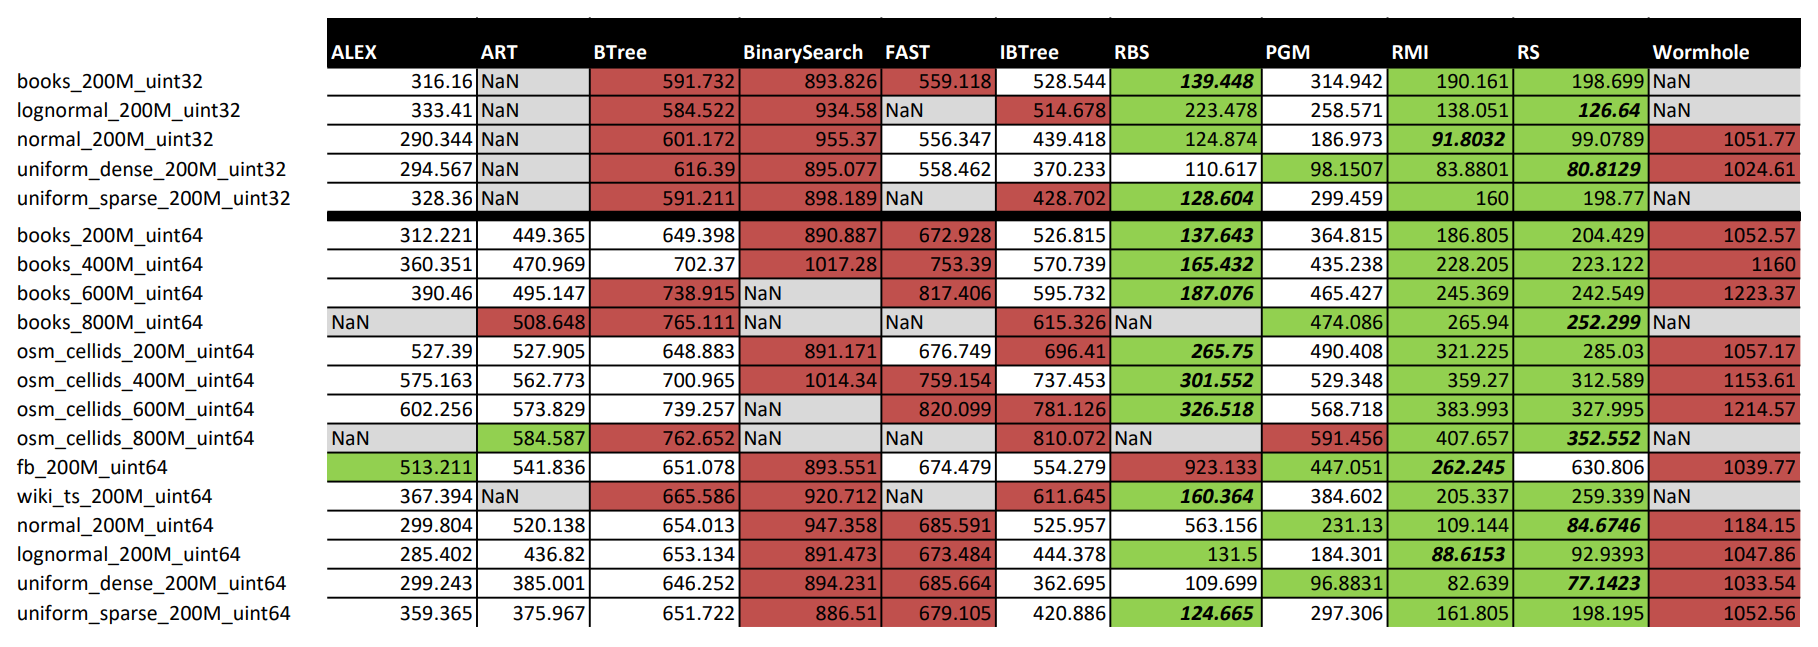
\includegraphics[width=1\textwidth]{sosd_lookups}
\caption[SOSD Lookups]{
  \textbf{SOSD lookup times (ns).}
  Lookup times produced by the benchmark when installed on our local test machine, selecting the best performing run with respect to the three metrics lookup time, build time and index size among all pareto runs.
}
\label{fig:sosd_lookups}
\end{figure}

\begin{figure}[ht]
\centering
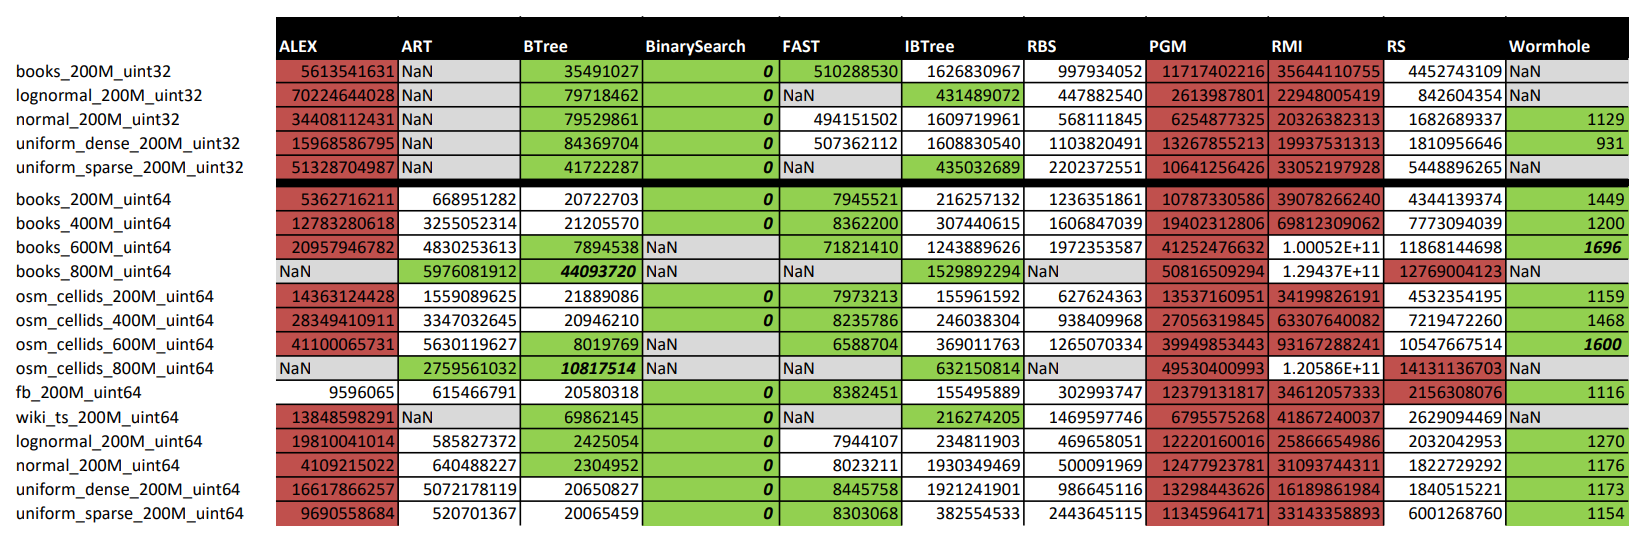
\includegraphics[width=1\textwidth]{sosd_builds}
\caption[SOSD Build Times]{
  \textbf{SOSD build times (ns).}
  Build times produced by the benchmark selected among pareto runs the same way as described above.
}
\label{fig:sosd_builds}
\end{figure}

\begin{figure}[ht]
\centering
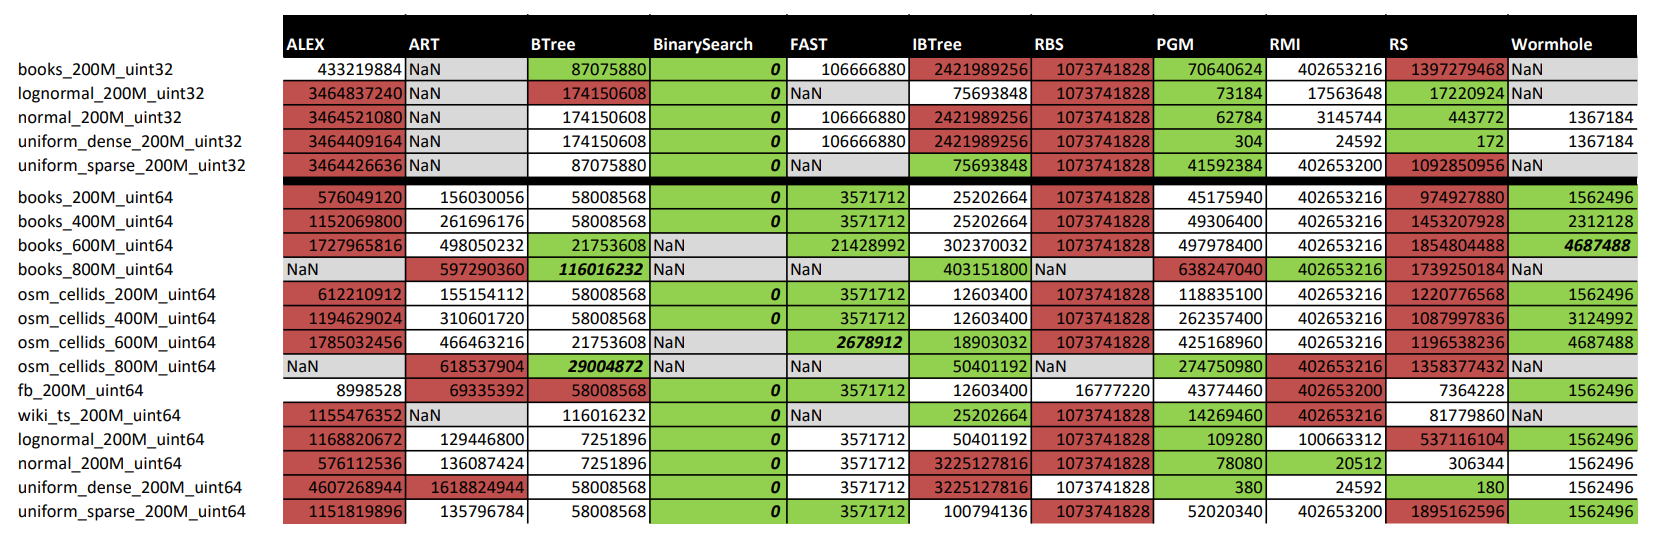
\includegraphics[width=1\textwidth]{sosd_sizes}
\caption[SOSD index sizes]{
  \textbf{SOSD index sizes (bytes).}
  Index sizes produced by the benchmark selected among pareto runs the same way as described above.
}
\label{fig:sosd_sizes}
\end{figure}


\section{Learned index structures}
In the benchmark there are currently three main competitors that belong to the category of learned index structures. Namely these are RMI, RS and PGM. RMI (Recursive Model Indexes) is proposed in \cite{rmi} and specificly implemented for the benchmark in \cite{cdfshop}. RS (Radix Spline) is proposed and implemented by the original authors in \cite{radixspline}. Finally PGM (Piecewise Geometric Model) is proposed in \cite{pgm} and also implemented by the authors.

\subsection{RMI: Recursive Model Indexes}
\label{sect:background:rmi}
RMI \cite{rmi} is a learned index structure that is based on the idea that different models fit certain data better. By having a number of different models to choose from during the learning phase and by allowing to stack different models on top of each other in different layers, RMI should adapt well to mostly any given shape of sorted data. In the context of the benchmark as well as in the context of this work, RMI's are fixed to two layers since this proved to be most efficient for most datasets and also reduces complexity for further chapters. In the concrete implementation in \cite{cdfshop} CDFShop generates C++ source files that contain parameters as well as the adapted code depending on which models where chosen on which layer. Generally the input key is fed into a first layer, which generates an index that then serves as a starting point for feeding the next layer, and so on, until finally a last layer retrieves the estimated key's position together with a stored error margin.\\
Notable for a potential P4 implementation here is that RMI is using floating point arithmetic, solely focussed on using the floating point FMA instruction. This immediately makes it a big challenge to think about implementing RMI in P4 but leaves some hope in the sense that if an FMA operation together with some simple form of floating point arithmetic could be implemented in P4 then RMI quite quickly would become realistic on a P4 device.

\subsection{RadixSpline: A Single-Pass Learned Index}
RS \cite{radixspline} is built on top of the idea of fitting a linear spline to the CDF of some sorted data. Different spline segments are indexed and to each segment two spline points are stored. Upon lookup the learned index tries to locate the responsible spline segment and performs a linear interpolation between the two spline points to find the estimated key position.\\
For P4 programmability important to note here is that RS stores the spline points in floating point format and upon lookup performs mathematical operations on these floating point numbers. The most notable operations in this context are the calculation of the slope of a spline segment which involves a floating point division and finally the interpolation itself which involves a floating point FMA instruction. This again makes it quite a big challenge to even start thinking about an RS implementation in P4. In comparision to RMI a big downside of RS is the part where the lookup code tries to locate the responsible spline segment. To make sure the correct segment is chosen either a linear search on small ranges or a binary search on bigger ranges is used. Both search concepts involve conditional iteration over dynamic data and are with that to my current knowledge far from easily feasible in P4.

\subsection{PGM: The Piecewise Geometric Model index}
PGM \cite{pgm} is a pure learned index structure that tries to create a piecewise linear approximation (PLA) that maps keys to their approximate positions in the data with at most $\epsilon$ distance to their actual position. By applying this approximation recursively onto itself multiple levels of PLA's are built such that efficient search becomes possible.\\
The given lookup code in \cite{pgm}, due to it's recursive nature at creation, needs to iterate over all levels of PLA for each lookup, which already marks a first challenge. To make things even harder in terms of P4 programmability on each level of PLA either linear search for small ranges or binary search for bigger ranges is used to determine which PLA is responnsible for a given key on the next level. This then results in a very similar situation as for RS, where a core concept used for looking up a key are far from easily feasible in P4 as described in the previous paragraph.

\section{P4 and network programmability}
P4 is a programming language that allows standardized programmability of network devices, especially targeting their packet forwarding planes. The language first appeared in 2013 and is since maintained by the P4 language consortium. Personally I was introduced to this language through my supervisor and further learned some of the basic concepts through the publicly available records of the P4 Developer Day held by \cite{p4-devday}. Annother important source for a deeper understanding of what the P4 language offers and which limitations exist is via the official specification by \cite{p4-spec}.\\
The idea behind learning P4 is to implement the best fitting of the previously presented learned index structures with the help of this language on a network device to satisfy our goal of resolving lookup requests directly through the network. The following preliminary facts need to be taken into consideration.

\begin{itemize}
  \item The P4 packet flow consists of different pipelines, inlcuding a packet parser, a checksum verification, an ingress pipeline, an egress pipeline, a checksum computation and finally a packet deparser.
  \item Parsers can have different states and allow transitions from state to state. States can loop back to other states but their logic must be reducable to a final state machine at compilation time, meaning there is no dynamic form of recursion or iteration allowed. (The only exception to this are header stacks where a packet can contain a dynamic but only up to a fixed amount of stack items that can be extracted through some form of state recursion)
  \item There are match-action tables that can optionally be filled with data from the control plane during runtime via P4Runtime. Tables allow matches on keys and execution of some specific action depending on the match.
  \item There is no possibility of linking P4 source files to each other similar as for example in C. This creates an environement where no major libraries exist, at most code snippets could be used.
  \item There is no notion of floating point numbers or arithmetic. The concepts do simply not exist in P4 land.
\end{itemize}

All together this leads to a very interesting language by itself but also to a rather cumbersome discovery of all that is actually not possible. Namely this means, especially in regard to what the different learned index structures implementations need, that in P4 there is no floating point arithmetic and there is no sort of loop or recursion capability.
